% This is sigproc-sp.tex -FILE FOR V2.6SP OF ACM_PROC_ARTICLE-SP.CLS
% OCTOBER 2002
%
% It is an example file showing how to use the 'acm_proc_article-sp.cls' V2.6SP
% LaTeX2e document class file for Conference Proceedings submissions.
% ----------------------------------------------------------------------------------------------------------------
% This .tex file (and associated .cls V2.6SP) *DOES NOT* produce:
%       1) The Permission Statement
%       2) The Conference (location) Info information
%       3) The Copyright Line with ACM data
%       4) Page numbering
%
%  However, both the CopyrightYear (default to 2002) and the ACM Copyright Data
% (default to X-XXXXX-XX-X/XX/XX) can still be over-ridden by whatever the author
% inserts into the source .tex file.
% e.g.
% \CopyrightYear{2003} will cause 2003 to appear in the copyright line.
% \crdata{0-12345-67-8/90/12} will cause 0-12345-67-8/90/12 to appear in the copyright line.
%
% ---------------------------------------------------------------------------------------------------------------
% It is an example which *does* use the .bib file (from which the .bbl file
% is produced).
% REMEMBER HOWEVER: After having produced the .bbl file,
% and prior to final submission,
% you need to 'insert'  your .bbl file into your source .tex file so as to provide
% ONE 'self-contained' source file.
%
% Questions regarding SIGS should be sent to
% Adrienne Griscti ---> griscti@acm.org
%
% Questions/suggestions regarding the guidelines, .tex and .cls files, etc. to
% Gerald Murray ---> murray@acm.org 
%
% For tracking purposes - this is V2.6SP - OCTOBER 2002

\documentclass[12pt]{article}
\setlength{\oddsidemargin}{0in}
\setlength{\evensidemargin}{0in}
\setlength{\topmargin}{0in}
\setlength{\headheight}{0in}
\setlength{\headsep}{0in}
\setlength{\textwidth}{6in}
\setlength{\textheight}{9in}
\setlength{\parindent}{0in} 

\usepackage{graphicx} %For jpg figure inclusion
\usepackage{times} %For typeface
\usepackage{epsfig}
\usepackage{color} %For Comments
\usepackage[all]{xy}
\usepackage{float}
\usepackage{subfigure} 
\usepackage{hyperref}
\usepackage{url}
\usepackage{parskip}



%% Elena's favorite green (thanks, Fernando!)
\definecolor{ForestGreen}{RGB}{34,139,34}
\definecolor{JoesGold}{RGB}{204,102,0}
% Uncomment this if you want to show work-in-progress comments
\newcommand{\comment}[1]{{\bf \tt  {#1}}}
% Uncomment this if you don't want to show comments
%\newcommand{\comment}[1]{}
\newcommand{\emcomment}[1]{\textcolor{ForestGreen}{\comment{Elena: {#1}}}}
\newcommand{\joecomment}[1]{\textcolor{JoesGold}{\comment{Joe: {#1}}}}
\newcommand{\todo}[1]{\textcolor{blue}{\comment{To Do: {#1}}}}
\newcommand{\hfcomment}[1]{\textcolor{Teal}{\comment{Henry: {#1}}}}
\newcommand{\clocode}[1]{{\texttt {#1}}}
%% Henry's color
\definecolor{Teal}{RGB}{2,132,130}

\begin{document}
\pagestyle{plain}
%
% --- Author Metadata here ---
%\conferenceinfo{WOODSTOCK}{'97 El Paso, Texas USA}
%\setpagenumber{50}
%\CopyrightYear{2002} % Allows default copyright year (2002) to be
%over-ridden - IF NEED BE. 
%\crdata{0-12345-67-8/90/01}  % Allows default copyright data
%(X-XXXXX-XX-X/XX/XX) to be over-ridden. 
% --- End of Author Metadata ---




\title{Exploration of parallelization efficiency in the Clojure programming language}
%\subtitle{[Extended Abstract \comment{DO WE NEED THIS?}]
%\titlenote{}}
%
% You need the command \numberofauthors to handle the "boxing"
% and alignment of the authors under the title, and to add
% a section for authors number 4 through n.
%
% Up to the first three authors are aligned under the title;
% use the \alignauthor commands below to handle those names
% and affiliations. Add names, affiliations, addresses for
% additional authors as the argument to \additionalauthors;
% these will be set for you without further effort on your
% part as the last section in the body of your article BEFORE
% References or any Appendices.




\author{
Henry Fellows, Joe Einertson, and Elena Machkasova \\
Computer Science Discipline \\
University of Minnesota Morris\\
Morris, MN 56267\\
??, eine0017@umn.edu, elenam@umn.edu
}




\date{}




\maketitle
\thispagestyle{empty}


\section*{\centering Abstract}
In modern processing environments, concurrency - simulationous execution of computations - is becoming an increasingly important tool in making gains in software performance. Despite the importance of parallelism, it is often poorly supported, or awkward to use effectively. Clojure is a Lisp dialect designed for concurrency and portability by Rich Hickey, first released in late 2007. Clojure runs on the Java Virtual Machine (JVM), and features immutable data structures and software transactional memory to make concurrent development easier. Immutable data structures do not present problems stemming from sharing the same memory. Clojure has proven to provide high efficiency of parallel processing. In 2012 \clocode{clojure.core.reducers} was added to the language: a novel library that contains a set of high level functions for an even more convenient and efficient parallel processing of data collections. 

In this study, we focus on testing the various methods of parallel processing in Clojure and explore the functionality of the reducers library. Timing the execution of computationally expensive and highly parallelizable data processing allows us to directly observe the differences between different methods of parallelism provided in Clojure. In order to time the execution we used a Clojure utility that allows access to the system clock. We created a function that records the system time, executes a given function, and then returns the elapsed time.
Reducers was found to provide a significant performance gain, in all situations, over \clocode{pmap}.  We present the results, analysis, and conclusions.
\emcomment{Apparently abstract needs to be under 150 words}


 \newpage
%this causes problems when compiling.

\setcounter{page}{1}


\section{Introduction}\label{sec:intro}

	Recently, Rich Hickey released a new library for the Clojure programming language that introduces major changes to the concurrency tools offered in Clojure's core library. Clojure is a dialect of Lisp, developed and first introduced in 2007 by Rich Hickey~\cite{Hickey:2008}, with a focus on concurrency and portability. By compiling into Java Bytecode, Clojure offers programmers ultra-portible code that leverages the widespread nature of the Java virtual machine. 

\section{Background}\label{sec:background}

\subsection{Clojure}\label{sec:clojure}
The Lisp family of languages has several features in common, the most visible of which is the polish-prefix notation. Cojure, as a Lisp, uses the polish-prefix notation, which can be generalized to \clocode{(function arg1 arg2 ... argN)}. For example, after interpretation, 
\begin{verbatim}
(+ 2 3)
=> 5
\end{verbatim}
Here \clocode{=>} denotes the Clojure interpreter response, so \clocode{(+ 2 3)}, when typed in the Clojure interpreter, evaluates to 5. 
Note that \clocode{+} in Clojure is a function, and not an operation, as in C or Java. 

Functions in Clojure are created using the \clocode{defn} macro, which has the basic syntax \clocode{(defn name [args] expr)}, where \clocode{name} is the function's name, \clocode{args} are function arguments listed with spaces in-between, and \clocode{expr} is the expression defining the behavior of the function. 
\begin{verbatim}
(defn add1 [num] (+ num 1))
(add1 4)
=> 5
\end{verbatim} 
%\emcomment{Walk the reader through the example: num is a parameter,  is a body, the next line is a function application.}
The first line in the above example defines the function \clocode{add1}, and the second line applies it to 4. In the first line \clocode{add1} marks the name of the function, \clocode{num} is the argument, and \clocode{(+ num 1)} is the expression.

Below we introduce vectors, an important Clojure data type for our discussion -- a type of collection in Clojure. Vectors are a collection of items, indexed by continuous integers: accessing items by index has a $O(log_{32}n)$  complexity. They are denoted by 
\clocode{[brackets]}.
\begin{verbatim}
(count [1 2 3 4 5])
=> 5
\end{verbatim}
\emcomment{explain what get does. Remember, most of your target audience have never seen a Lisp-like language}
Lisps have a philosophy of treating code as data, meaning that all functions can take functions (or other code) as arguments. Because of that philosophy, most Lisps, including Clojure, provide a rich set of higher-order functions that allow for powerful manipulation of data. Clojure includes \clocode{map}, a function that takes a function and a collection and then applies the function to every item in the collection, returning the resulting collection. The type of the collection that gets returned is not a vector, but a more general collection type, so it is included in parentheses, and not brackets. However, for the most part this distinction is not important for our discussion. 
%\emcomment{A seq is not, strictly speaking, a concrete type. I also think this sentence is confusing to readers. Perhaps saying that what gets returned is not a vector, but a more general type of a collection, known as a sequence?}
\begin{verbatim}
(map add1 [0 1 2 3 4])
=>(1 2 3 4 5)
\end{verbatim}

Clojure pre-defined functions include \clocode{reduce}, also known as fold in other Lisps, which recursively applies the function to the first element of a collection and the result of applying a reduce to the rest of the collection, repeating this process until the collection is empty.
\begin{verbatim}
(reduce + [1 2 3])
=> 6
\end{verbatim}
The next of the major high-order functions is \clocode{filter}, which takes a predicate (a function that returns a boolean and has no side-effects) and a collection and returns a new collection of the items in the original collection for which the predicate (when applied to the item) returns true.
\begin{verbatim}
(filter even? [1 2 3 4 5])
=> (2 4)
\end{verbatim}
Another common feature in clojure is laziness. Laziness is the concept of delaying evaluation of an expression untill the value it returns is needed.
\emcomment{Explain the concept of laziness since you use it later}

\subsection{Introduction to concurrency}\label{sec:concurrency}
 Lately, processor clock speed has plateaued - simply running the CPU faster - is no longer a viable option in the eyes of hardware designers.
\emcomment{The grammatical structure of this sentence needs to change.}
In order to maintain throughput growth, processors are now being built with multiple cores. In order to be able to effectively use modern processors, programmers must begin to use concurrency. Concurrency is simply the execution of multiple computations simultaneously. Most programming languages support concurrent programming, but many provide poor support, or have awkward interfaces. 

Programming concurrent programs is hard, especially the issue of shared resources (commonly memory). Simply speaking, having two parts of a program access one resource at the same time can casue problems. Modern concurrency systems use some sort of access management to prevent this, by giving one thread exclusive access to a resouce while the thread reads or writes to it. Unfortunately, this model can cause problems such as deadlocking, where two tasks are waiting for resources that the other task holds. If not resolved, both threads will wait forever. In contrast to this model, Clojure uses Software Transactional Memory. STM is a method of managing shared resources without using locking; every thread can modify a shared resource without regard for the action of other threads. When a thread accesses a resource, it records it's actions in a log; near the end of the transaction, is checks to see if another thread has modified the resouce. If the resource has been accessed, it restarts, and attempts to successfully modify the resource again.

Clojure uses immutable datatypes by default; the value of an immutable datatype cannot be changed after it has been created. New copies of an object are created every time the object is modified, making it impossible for threads to modify objects as they are read. is immutable and this allows concurrency to be added to programs that were not designed for concurrency without any major redesign. Additionally, Clojure provides drop-in replacements for the built in higher order functions (discussed above) that allow programmers not familiar with concurrency to use concurrency in their programs.
\emcomment{Need to mention that in cases when mutation is required, Clojure provides several types of access that vary in degree of synchronization of access among multiple threads.}\hfcomment{I don't know about that side of Clojure - I'll leave it to you.}
\emcomment{Will do}


\subsection{Introduction to pmap}\label{sec:pmap}
\clocode{pmap} was an early attempt at providing a parallel version of map; with the same arguements as \clocode{map}, \clocode{pmap} is a drop-in replacement. 
\begin{verbatim}
(pmap add1 [1 2 3 4])
=> (2 3 4 5)
\end{verbatim}
Importantly, \clocode{pmap} is semi-lazy; it tries to use as little processing as possible, only returning results as needed ; that is, it can occassionally appear to evaluate as a serial function.\emcomment{This is ambiguous: I think you mean as little processing as possible, but it reads like it's trying to work sequentially}. If the value is used (by a function, for example), pmap will evaluate the entire expression immediately (i.e eager evaluation), and always in parallel. \clocode{doall} in Clojure forces eager evaluation on lazy expressions. In all of our tests, \clocode{doall} is used to force eager evaluation. If we imagine a long running function, \clocode{expensive-function}, we can time it and see the difference \clocode{doall} makes.
\begin{verbatim}
(time (pmap expensive-function [1 2 3 4]))
=> 12000 ms 
;because doall forces eager evaluation, it runs faster - roughly by a factor of the number of cores (in this case, four).
(time (doall (pmap  expensive-function  [1 2 3 4])))
=> 3000 ms
\end{verbatim}

 \emcomment{doall is one way of forcing evaluation; you should mention that if a result is used (e.g. by reduce) then it would evaluate. }


\subsection{Introduction to reducers}\label{sec:reducers}
Reducers library was released by Rich Hickey in May 2012~\cite{HickeyReducers}. Reducers provides higher-order functions for the manipulation of collections, focusing on concurrent versions of the native high-order functions.  Built on Java's ForkJoin framework, Reducers uses the same data structures as the original functions, allowing drop-in replacement for many use cases.
\emcomment{Elena's section}

\section{Efficiency of parallel methods in Clojure}\label{sec:efficiency} 

\subsection{Test structure}\label{sec:testStruct}
To determine the performance implications of the new reducers library, we have split each of our tests into two sections. First, we run the test using Clojure's multi-threaded reduce, r/fold, which computes the entire result in one operation. Then, we run the test using a two-step process: first, a map operation which prepares values for reduction, followed by a reduce operation which combines the values computed in the first step. This two-step method allows us to shift where and how the most processing power is used, and to determine what combination of elements is most efficient.
\emcomment{While this does indeed describe our tests, I wonder if we can make it clearer by using an itemized list or a table or some such: it's *very* difficult to get this information from reading this paragraph. We also do r/fold + r/map, I am not sure it is included here.}\joecomment{Might make sense to have a table of all operations - name, "type" (map vs reduce) and whether it is single- or multi-threaded?}
The tests are summarized in table~\ref{table:tests}.

\begin{table}
\begin{center}
\begin{tabular}{|l|l|}
\hline 
Name & Description \\
\hline
map + reduce & serial map, serial reduce \\
pmap + reduce & parallel map, serial reduce \\
\hline
\end{tabular}
\end{center}
\caption{Configurations for our tests}\label{table:tests}
\end{table}

The one-step testing method is always multi-threaded, using the new reducers library. \emcomment{In the table it's easier to refer to these cases as parallel and serial. Would it be reasonable to use this in the text as well?} The two-step method tests all combinations of single- and multi-threaded, using both serial map and reduce, as well as parallel pmap, r/map and r/fold. We call each unique combination of functions a \emph{configuration}. Configurations, in turn, make up the two sections described, and those sections comprise the overall test.\emcomment{The previous paragraph and this one should be combined and streamlined: it would be better to introduce the term "configuration" first, and then discuss various configurations.}

Since the requirements for parallelizing reduce are more strict than for parallelizing map, this many-part methodology allows us to analyze not only running time, but also to determine whether parallel reduction offers such a speedup over single-threaded or parallel map-based solutions so as to warrant the additional overhead of coding it. \emcomment{I really don't think this is an issue: it's really not involved at all}

When executing a test, each configuration is run on the same set of data. Additionally, each test is run many times on different data.
\emcomment{These two sentences are confusing. We run each test on the same randomly generated data in each configuration, and we repeat this process many(?) times?} 
The input data used for all three tests we describe consists of large collections of very large, uniformly distributed, randomly generated integers. The exact specifications for each test are listed in Table X \todo{Reference the table once it exists}\joecomment{Henry - Please correct if this is wrong in some way.}
\emcomment{It would be better to reference the table earlier and walk the reader through it in this section}

\subsection{Fermat primality test}\label{sec:fermat}
Two of the tests described are centered on determining which numbers in the collection are prime. Specifically, we use a probabilistic algorithm called the \emph{Fermat primality test}, which takes two parameters: a number to test for primality, and an integer that determines the number of trials to be run. The higher the number of trials, the more precise the result and the more processing power used. We set the maximum number of trials per number to 5 trials, which gives a high degree of accuracy for a moderate amount of processing power. Fermat primality test is used for very large numbers since faster algorithms exist for smaller numbers. We use numbers on the order of \emcomment{Need to fill this in}
%\emcomment{is it up to 5? Because if it's composite, it may finish earlier, right?}\joecomment{True, although I'm not sure that distinction is useful for this paper. I think that may introduce confusion.}

The Fermat primality test relies heavily on exponentiation and modular arithmetic, operations which are relatively expensive for large numbers (we use integers between zero and one billion). The specific mathematics behind the Fermat primality test are tangential to and beyond the scope of this paper. The reasons this test was chosen is 
%It is only necessary to understand that we chose this test 
because it is simple to implement, computationally expensive, and an example of a real-world operation which may benefit from Clojure's reducers. 
%These assertions all hinge on the fact that we use the Fermat primality test on large numbers (for small numbers, there are faster primality tests).
%\emcomment{Would it be useful to mention that the test makes calls to Java library functions and uses bigint (if it indeed uses bigints)?}\joecomment{Maybe. That seems like too much detail, but I could see an argument the other way too. I'm impartial.}

\subsubsection{Compare-Count-Primes}\label{sec:count-primes}
The first test we describe is an algorithm to determine the number of prime integers in a  collection of integers. In the one-step implementation described above, we use a simple reduce operation to count the number of primes:

\begin{verbatim}
(defn reduce-num-primes [a b] 
   (if (p/fermat-test b 5)
         (inc a)
         a))
\end{verbatim}

Simply, for each element which is found to be prime via the Fermat primality test, we increase the running sum of primes by one (starting from 0). This implementation leverages r/fold, meaning it is a parallel reduce operation. 
\emcomment{Need to explain what a and b are and other notations (p/fermat-test, have we defined inc?) }

As described previously, we also tested the pure r/fold implementation against configurations that used varying combinations of reduction and mapping functions. In these cases, we used this mapping function:

\begin{verbatim}
(defn count-primes-pre-reducer [x] 
    (if (p/fermat-test x 5) 1 0))
\end{verbatim}

Here the work of determining the primality of the numbers is moved into a mapping operation, which returns 1 for each element if prime, or 0 if not. Then we use r/fold to sum the result in parallel. This is simpler from an implementation standpoint, as our mapping function does not have to conform to the restrictions of r/fold, and summation is trivial to use with r/fold.\joecomment{Is this redundant now with the section describing our test structure?}

The data used for this test is a collection of 100,000 random integers uniformly distributed between 0 and 1 billion. This test was run 100 times. \joecomment{Does this belong in a table? If so, someone else want to do it? :) Never done a LaTeX table and not too excited to learn...}
\emcomment{Yes -- No (I don't want to) -- will do.}

  
\subsubsection{Compare-Sum-Primes}\label{sec:sum-primes}
The second test we describe is broadly similar to compare-count-primes, but sums the value of all primes (ignoring composite numbers) rather than simply counting them. This is a more computationally expensive test, since the numbers being \emph{summed} are very large, rather than 0's and 1's. The purpose of this test is to add computational complexity to the r/fold portion to determine what effect the distribution of work has on running time.

First, there is our basic, all-in-one reduce function:

\joecomment{We may want to describe + vs +' in Clojure prior to this}
\begin{verbatim}
(defn reduce-sum-primes [a b]
  (if (p/fermat-test b 5)
         (+' a b)
         a))
\end{verbatim}

The mapping function used during the second stage of testing is similarly simple:

\begin{verbatim}
(defn sum-primes-pre-reducer [x] 
    (if (p/fermat-test x 5) x 0))
\end{verbatim}

This test also used a collection of 10,000 random integers uniformly distributed between 0 and 1 billion, but was run 1,000 times.
 
\subsubsection{Compare-Sum-Sqrt}\label{sec:sum-sqrt}
 
The final test we describe utilizes another computationally-expensive algorithm: integer square root. This method of computing a square root returns the floor of the exact square root of a number. Like computing primality, calculating integer square roots is a computationally difficult task, which represents a good opportunity to utilize and measure parallelism. 

To calculate the integer square root, we use a Clojure math library, Clojure Numeric Tower. In our code, we refer to this library as "cljmath."

This test is a straightforward "calculate-and-sum" algorithm, and as such its one-pass reduce function is very basic:

\begin{verbatim}
(defn reduce-sum-sqrt [a b] 
    (+' a (cljmath/sqrt b)))
\end{verbatim}

For the multi-step configurations, our map function is simply the \texttt{cljmath/sqrt} function - we calculate the square root as the map step, and sum the square roots as the reduce step.
 
This test used a collection of 100,000 random integers uniformly distributed between 0 and 1 billion, and was run 1,000 times.
 
 \subsection{Execution Methodology}\label{sec:eMethods}
 Following the methods shown above, we ran the tests on several different machines referred to as box1, box2, and box3.
 
\begin{itemize}
 \item 
 Box 1 has an Intel i7 (4700MQ) cpu, with 4 hyperthreaded cores, running Windows 7.
 \item
 Box 2 has an Intel i5 (650) cpu, with 4 cores, running Fedora 18.
 \item
 Box 3 has an AMD FX-8350 cpu, with 8 cores, running Fedora 18. 
 \end{itemize}
  
The full set of tests was run three times on each machine. The first run is discarded due to Java virtual machine warm-up, a period where the program runs significantly slower than it would normally ~\cite{Blackburn:2008} . This period is caused by the JVM preforming dynamic optimization and lazy loading relevant portions of code. In order to provide data that is unambiguous and easy to interpret, we omit that portion of the data from the results. It is important to note that the ratio between each portion of a test remained constant.

\emcomment{Need to explain why we aren't using a filter here for primality testing examples: for consistency with pmap?}

\subsection{Results}\label{sec:results}
In this section we show the results of running our tests across the machines mentioned above;

\begin{table}
\begin{center}
\begin{tabular}{|l|c|c|c|c|c|c|}
\hline
Machine & reduce + map & reduce + pmap & r/fold + map & r/fold + pmap & r/fold & r/fold + r/map \\
\hline
Box 1 & 208.0 & 66.4 & 61.7 & 207.0 & 57.2 &  54.6 \\
Box 2 & 279.3 & 250.6 & 284.3 & 280.8 & 132.0 & 131.0 \\
Box 3 & 266.9 & 225.1 & 248.4 & 275.5 & 59.2 & 63.6 \\
\hline
\end{tabular}
\end{center}
\caption{Sum-Primes Averages.}\label{table:sum-primes}
\end{table}

\begin{table}
\begin{center}
\begin{tabular}{|l|c|c|c|c|c|}
\hline
Machine & reduce + map & reduce + pmap & r/fold + map & r/fold + pmap & r/fold\\
\hline
Box 1 & 2084.6 & 604.5 & 597.1 & 2065.7 & 535.8\\
Box 2 & 2567.7 & 2585.6 & 2774.0 & 1269.3 & 1269 \\
Box 3 & 2411.3 & 2426.6 & 2647.9 & 562.9 & 557.6\\
\hline
\end{tabular}
\end{center}
\caption{Count-Primes Averages.}\label{table:sum-primes}
\end{table}

\begin{table}
\begin{center}
\begin{tabular}{|l|c|c|c|c|c|}
\hline
Machine & reduce + map & reduce + pmap & r/fold + pmap & r/fold + r/map & r/fold\\
\hline
Box 1 & 115.4 & 128.7 & 109.7 & 28.6 & 30.5\\
Box 2 & 120.1 & 401.3 & 414.0 & 60.0 & 58.0 \\
Box 3 & 115.9 & 359.5 & 367.6 & 32.8 & 32.4\\
\hline
\end{tabular}
\end{center}
\caption{Sum-Sqrt Averages.}\label{table:sum-primes}
\end{table}

A typical mode was to find that the distributon was in two peaks - the serial methods and the parallel methods; 

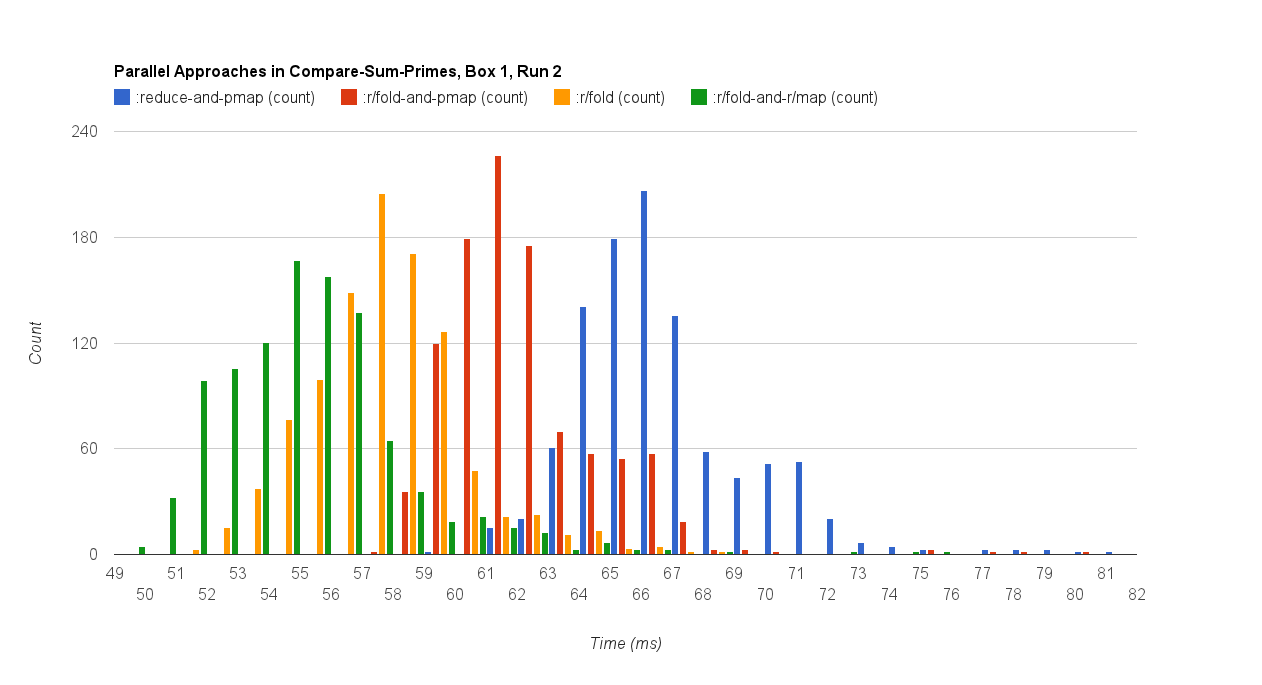
\includegraphics[trim = 10mm 0mm 30mm 0mm, clip, width = 16cm,height = 10cm]{PSP-B1}
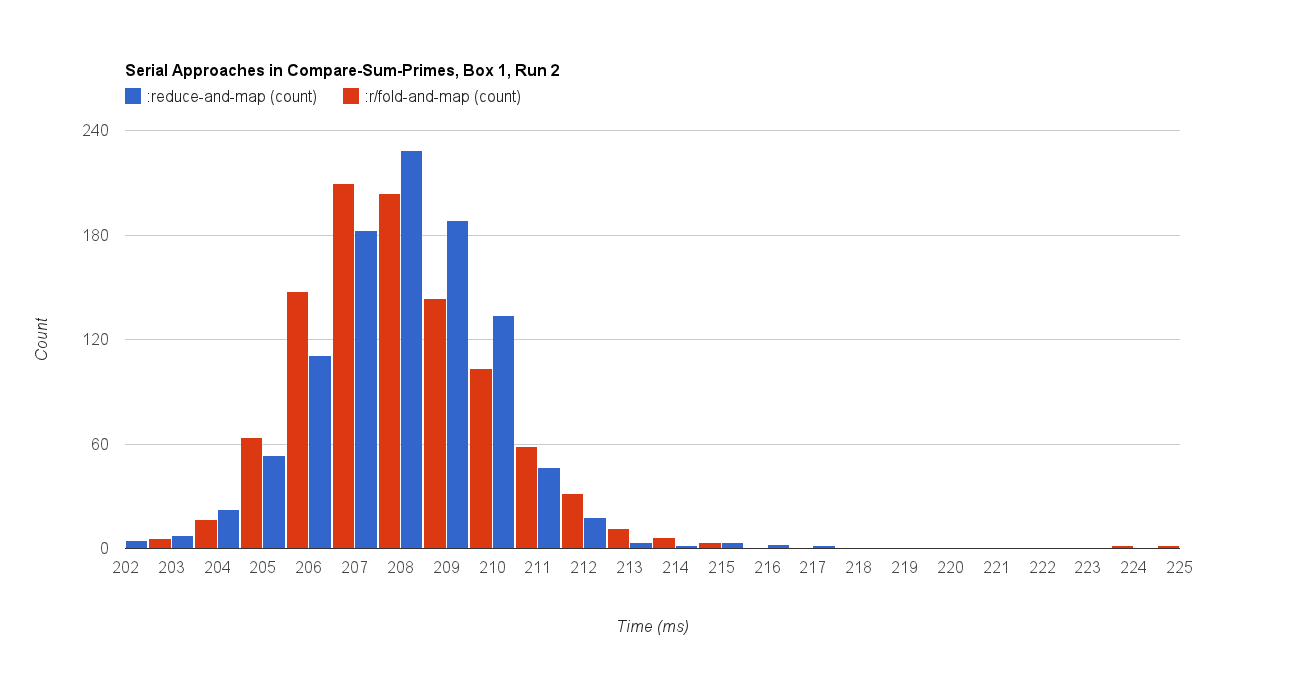
\includegraphics[trim = 10mm 0mm 0mm 5mm, clip, width = 16cm,height = 11cm]{SSP-B1}



\subsection{Discussion}\label{sec:discussion}
We have found that the reducers library, in all tested cases, reduces the execution time significantly. In both Intel machines, the reduction was close to a factor of the number of cores. The AMD Fx-8350 machine tested did not show this same pattern - We suspect that the somewhat novel Bulldozer architecture, where each pair of cores are packaged into modules that share components ~\cite{McIntyre:2012} was a factor. \clocode{pmap}, when properly executing in parallel was somewhat slower, but was often executing in serial time. In several instances \clocode{pmap} was up to x\% slower than serial methods. We briefly looked into the cause, but were unable to gather a statistically significant amount of data. What data we do have points to a large amount of threads being created, leading to excessive context switching. 

\section{Conclusions and future work}\label{sec:conclusion}




\subsection{Future Work}\label{sec:future}








%
% The following two commands are all you need in the
% initial runs of your .tex file to
% produce the bibliography for the citations in your paper.
%\bibliographystyle{abbrv}
%\end{thebibliography}




%\bibliography{generic_types}  
% You must have a proper ".bib" file
%  and remember to run:
% latex bibtex latex latex
% to resolve all references
%
% ACM needs 'a single self-contained file'!
%
\bibliographystyle{abbrv}
\bibliography{mics2014reducers}








% That's all folks!
\end{document}

%%%%%%%%%%%%%%%%%%%%%%%%%%%%%%%%%%%%%%%%%%%%%%%%%%%%%%%%%%%%%%%%
